\documentclass[journal]{IEEEtran}
\usepackage[a5paper, margin=10mm]{geometry}
%\usepackage{lmodern} % Ensure lmodern is loaded for pdflatex
\usepackage{tfrupee} % Include tfrupee package


\setlength{\headheight}{1cm} % Set the height of the header box
\setlength{\headsep}{0mm}     % Set the distance between the header box and the top of the text


%\usepackage[a5paper, top=10mm, bottom=10mm, left=10mm, right=10mm]{geometry}

%
\setlength{\intextsep}{10pt} % Space between text and floats

\makeindex


\usepackage{cite}
\usepackage{amsmath,amssymb,amsfonts,amsthm}
\usepackage{algorithmic}
\usepackage{graphicx}
\usepackage{textcomp}
\usepackage{xcolor}
\usepackage{txfonts}
\usepackage{listings}
\usepackage{enumitem}
\usepackage{mathtools}
\usepackage{gensymb}
\usepackage{comment}
\usepackage[breaklinks=true]{hyperref}
\usepackage{tkz-euclide} 
\usepackage{listings}
\usepackage{multicol}
\usepackage{xparse}
\usepackage{gvv}
%\def\inputGnumericTable{}                                 
\usepackage[latin1]{inputenc}                                
\usepackage{color}                                            
\usepackage{array}                                            
\usepackage{longtable}                                       
\usepackage{calc}                                             
\usepackage{multirow}                                         
\usepackage{hhline}                                           
\usepackage{ifthen}                                               
\usepackage{lscape}
\usepackage{tabularx}
\usepackage{array}
\usepackage{float}
\usepackage{ar}
\usepackage[version=4]{mhchem}


\newtheorem{theorem}{Theorem}[section]
\newtheorem{problem}{Problem}
\newtheorem{proposition}{Proposition}[section]
\newtheorem{lemma}{Lemma}[section]
\newtheorem{corollary}[theorem]{Corollary}
\newtheorem{example}{Example}[section]
\newtheorem{definition}[problem]{Definition}
\newcommand{\BEQA}{\begin{eqnarray}}
\newcommand{\EEQA}{\end{eqnarray}}

\theoremstyle{remark}


\begin{document}
\bibliographystyle{IEEEtran}
\onecolumn

\title{12.561}
\author{INDHIRESH S- EE25BTECH11027}
\maketitle


\renewcommand{\thefigure}{\theenumi}
\renewcommand{\thetable}{\theenumi}

\textbf{Question}.The following system of equations
\begin{align*}
    2x-y-z=0\\
    -x+2y-z=0\\
    -x-y+2z=0
\end{align*}
\begin{enumerate}
    \item has no solution
    \item  has a unique solution
    \item  has three solutions.
    \item has an infinite number of solutions
\end{enumerate}
\textbf{Solution}:\\
Let us solve the given equation theoretically and then verify the solution computationally. \\
The given eqaution can be given as:
\begin{align}
 \Vec{A}\Vec{x}=\Vec{B}
\end{align}


\begin{align}
  \myvec{2&-1&-1\\-1&2&-1\\-1&-1&2}\Vec{x}=\myvec{0\\0\\0}
\end{align}
Now forming the augmented matrix and performing row operations
\begin{align}
   \augvec{3}{2}{2&-1&-1&0\\-1&2&-1&0\\-1&-1&2&0}\xleftrightarrow{R_1\longleftarrow R_2}\augvec{3}{2}{-1&2&-1&0\\2&-1&-1&0\\-1&-1&2&0}
\end{align}

\begin{align}
  \augvec{3}{2}{-1&2&-1&0\\2&-1&-1&0\\-1&-1&2&0}\xleftrightarrow{R_3\longleftarrow R_3-R_1}\augvec{3}{2}{-1&2&-1&0\\0&3&-3&0\\0&-3&3&0}
\end{align}

\begin{align}
\augvec{3}{2}{-1&2&-1&0\\0&3&-3&0\\0&-3&3&0}\xleftrightarrow{R_3\longleftarrow R_3+R_2}\augvec{3}{2}{-1&2&-1&0\\0&3&-3&0\\0&0&0&0}
\end{align}

Here the rank of the matrix is 2 which is less than 3.\\
So the system of the equation has an infinite number of solutions

From the figure it is clearly verified that the theoretical solution matches with the computational solution.\\
\begin{figure}[h]
    \centering
    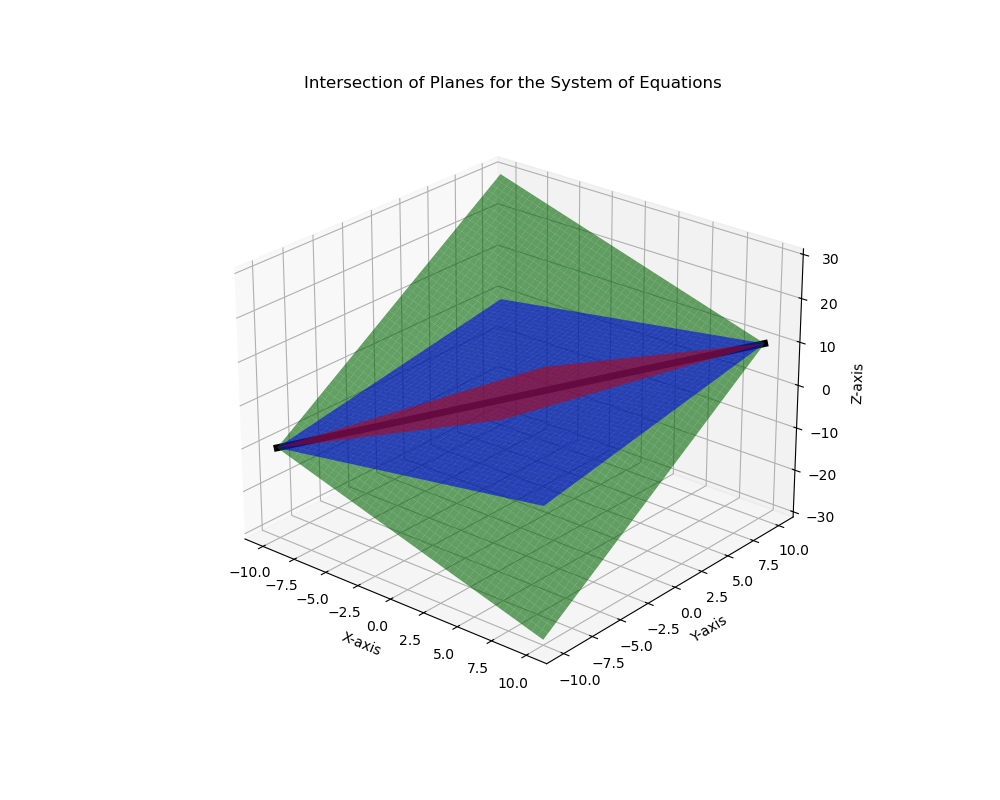
\includegraphics[height=0.5\textheight, keepaspectratio]{figs/figure1.png}
    \label{figure_1}
\end{figure}

\end{document}